%\documentclass[convert={density=300,size=800x800,outext=.png}]{standalone}
\documentclass{article}
\usepackage{amsmath, tikz}

\DeclareMathOperator{\im}{im}

\begin{document}
\section{first-1}
\begin{center}
	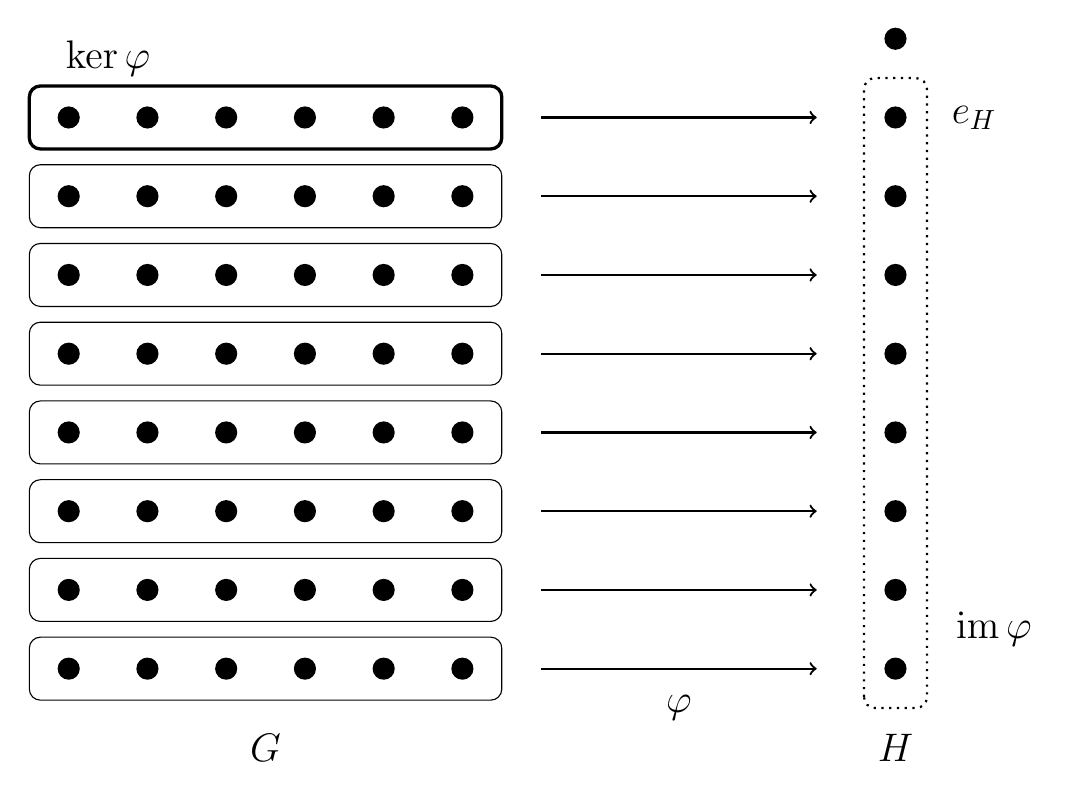
\begin{tikzpicture}
		% elements of G
		\foreach \x in {0,...,5}
		\foreach \y in {0,...,7}
		{
			\fill (\x+0.5,\y+0.5) circle (4pt);
		}
		\node at (3,-0.5) {\Large{$G$}};
		% cosets of \ker\varphi
		\foreach \x in {0,...,7}
		{
			\draw[rounded corners] (0,\x+0.1) rectangle (6,\x+0.9);
		}
		% bold subgroup \ker\varphi
		\draw[rounded corners, very thick] (0,7.1) rectangle (6,7.9);
		% arrows of \varphi
		\foreach \x in {0,...,7}
		{
			\draw[->, thick] (6.5,\x+0.5) -- (10,\x+0.5);
		}
		\node at (8.25,0) {\Large{$\varphi$}};
		% elements of H
		\foreach \x in {0,...,8}
		{
			\fill (11,\x+0.5) circle (4pt);
		}
		% highlight subgroup \im\varphi
		\draw[rounded corners, dotted, thick] (10.6,0) rectangle (11.4,8);
		\node at (11,-0.5) {\Large{$H$}};
		% other labels
		\node at (1,8.25) {\Large{$\ker\varphi$}};
		\node at (12.25,1) {\Large{$\im\varphi$}};
		\node at (12,7.5) {\Large{$e_H$}};
	\end{tikzpicture}
\end{center}

\section{first-2}
\begin{center}
	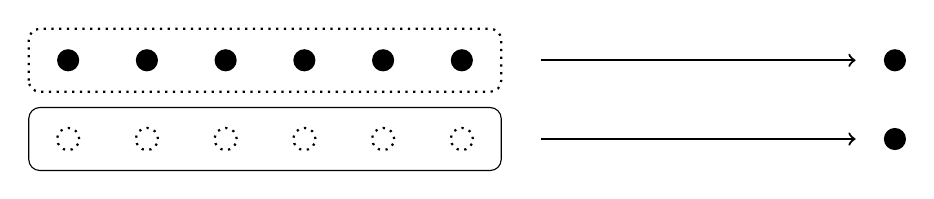
\begin{tikzpicture}
		% elements of G
		\foreach \x in {0,...,5}
		{
			%\fill (\x+0.5,0.5) circle (4pt);
      \draw[dotted, thick] (\x+0.5,0.5) circle (4pt);
			\fill (\x+0.5,1.5) circle (4pt);
		}
		% boxes around elements of G
		\draw[rounded corners] (0,0.1) rectangle (6,0.9);
		\draw[rounded corners, dotted, thick] (0,1.1) rectangle (6,1.9);
		% arrows of \varphi
		\draw[->, thick] (6.5,0.5) -- (10.5,0.5);
		\draw[->, thick] (6.5,1.5) -- (10.5,1.5);
		% elements of H
		\fill (11,0.5) circle (4pt);
		\fill (11,1.5) circle (4pt);
	\end{tikzpicture}
\end{center}

\section{second-1}
\begin{center}
	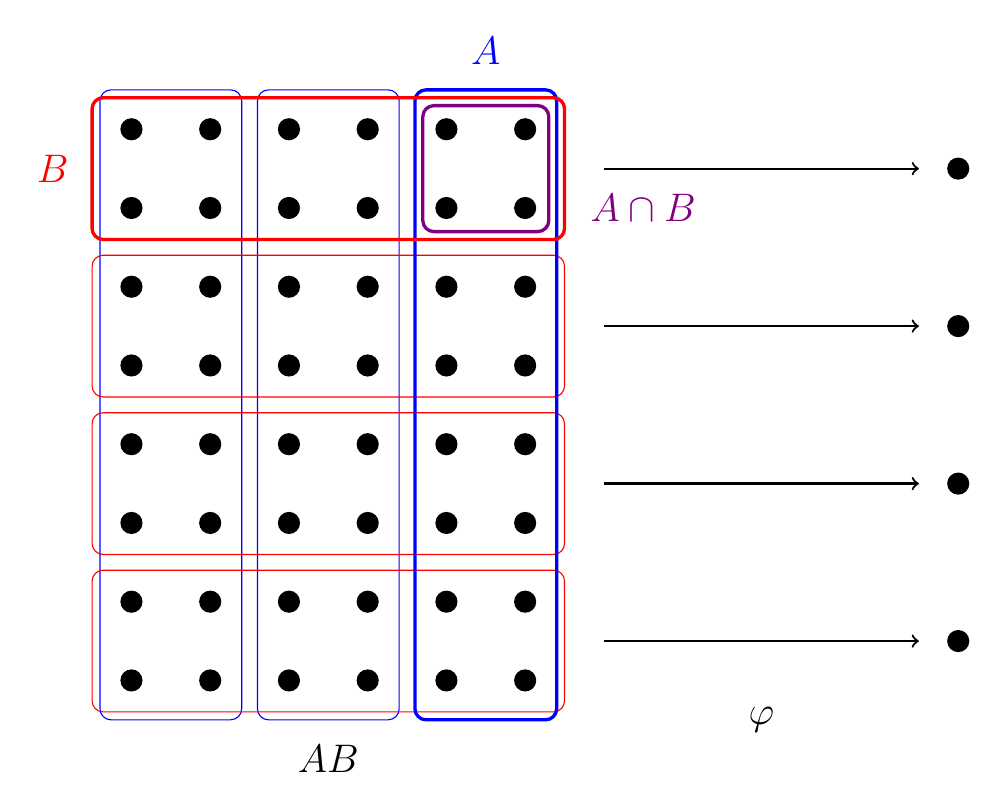
\begin{tikzpicture}
		% elements of AB
		\foreach \x in {0,...,5}
		\foreach \y in {0,...,7}
		{
			\fill (\x+0.5,\y+0.5) circle (4pt);
		}
		% cosets of A
		\foreach \x in {0,...,2}
		{
			\draw[rounded corners, blue] (2*\x+0.1,0) rectangle (2*\x+1.9,8);
		}
		% cosets of B
		\foreach \y in {0,...,3}
		{
			\draw[rounded corners, red] (0,2*\y+0.1) rectangle (6,2*\y+1.9);
		}
		% box elements of A \cap B
		\draw[rounded corners, very thick, violet] (4.2,6.2) rectangle (5.8,7.8);
		% bold subgroups A and B
		\draw[rounded corners, very thick, blue] (4.1,0) rectangle (5.9,8);
		\draw[rounded corners, very thick, red] (0,6.1) rectangle (6,7.9);
		% arrows of \varphi
		\foreach \x in {0,...,3}
		{
			\draw[->, thick] (6.5,2*\x+1) -- (10.5,2*\x+1);
		}
		\node at (8.5,0) {\Large{$\varphi$}};
		% elements of H
		\foreach \x in {0,...,3}
		{
			\fill (11,2*\x+1) circle (4pt);
		}
		% other labels
		\node at (3,-0.5) {\Large{$AB$}};
		\node[blue] at (5,8.5) {\Large{$A$}};
		\node[red] at (-0.5,7) {\Large{$B$}};
		\node[violet] at (7,6.5) {\Large{$A\cap B$}};
	\end{tikzpicture}
\end{center}

\section{second-2}
\begin{center}
	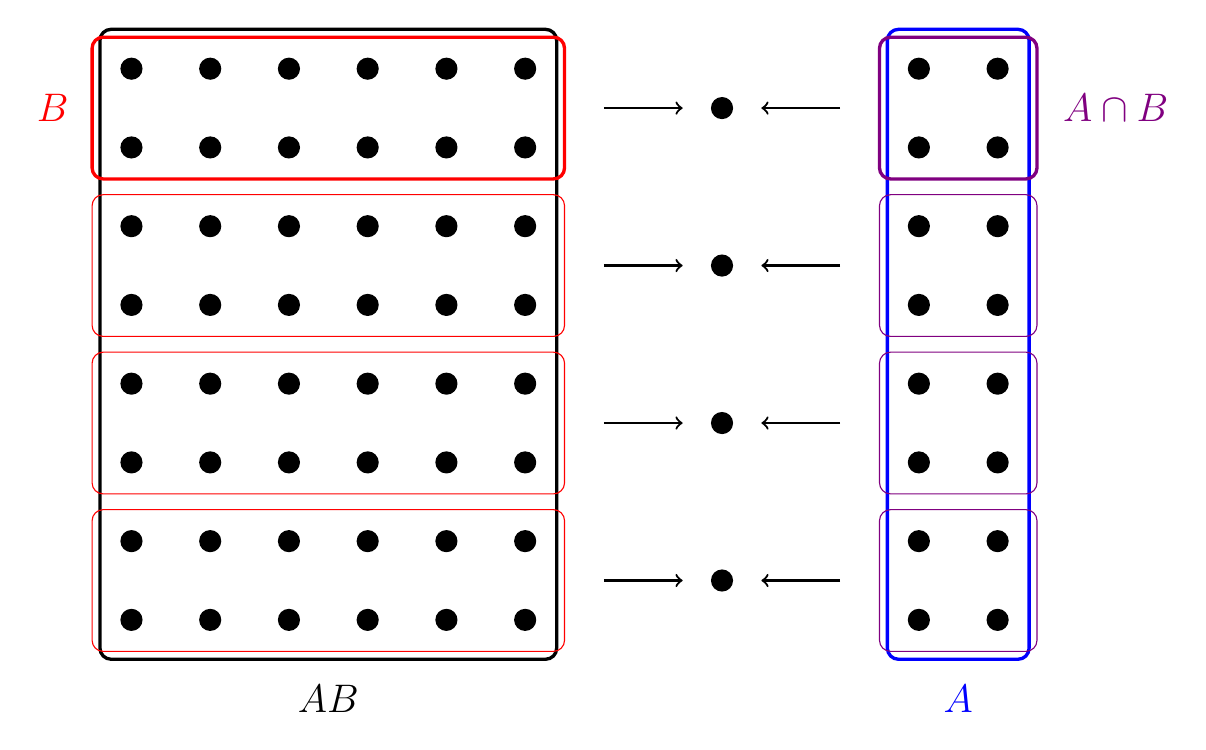
\begin{tikzpicture}
		% elements of AB
		\foreach \x in {0,...,5}
		\foreach \y in {0,...,7}
		{
			\fill (\x+0.5,\y+0.5) circle (4pt);
		}
		% bold subgroup AB
		\draw[rounded corners, very thick] (0.1,0) rectangle (5.9,8);
		% cosets of B
		\foreach \y in {0,...,3}
		{
			\draw[rounded corners, red] (0,2*\y+0.1) rectangle (6,2*\y+1.9);
		}
		% bold subgroup B
		\draw[rounded corners, very thick, red] (0,6.1) rectangle (6,7.9);
		% arrows of \varphi on the left side
		\foreach \x in {0,...,3}
		{
			\draw[->, thick] (6.5,2*\x+1) -- (7.5,2*\x+1);
		}
		% elements of H
		\foreach \x in {0,...,3}
		{
			\fill (8,2*\x+1) circle (4pt);
		}
		% arrows of \varphi on the right side
		\foreach \x in {0,...,3}
		{
			\draw[->, thick] (9.5,2*\x+1) -- (8.5,2*\x+1);
		}
		% elements of A
		\foreach \x in {0,...,1}
		\foreach \y in {0,...,7}
		{
			\fill (\x+10.5,\y+0.5) circle (4pt);
		}
		% bold subgroup A
		\draw[rounded corners, very thick, blue] (10.1,0) rectangle (11.9,8);
		% cosets of A \cap B
		\foreach \y in {0,...,3}
		{
			\draw[rounded corners, violet] (10,2*\y+0.1) rectangle (12,2*\y+1.9);
		}
		% bold subgroup A \cap B
		\draw[rounded corners, very thick, violet] (10,6.1) rectangle (12,7.9);
		% other labels
		\node at (3,-0.5) {\Large{$AB$}};
		\node[blue] at (11,-0.5) {\Large{$A$}};
		\node[red] at (-0.5,7) {\Large{$B$}};
		\node[violet] at (13,7) {\Large{$A\cap B$}};
	\end{tikzpicture}
\end{center}

\section{third-1}
\begin{center}
	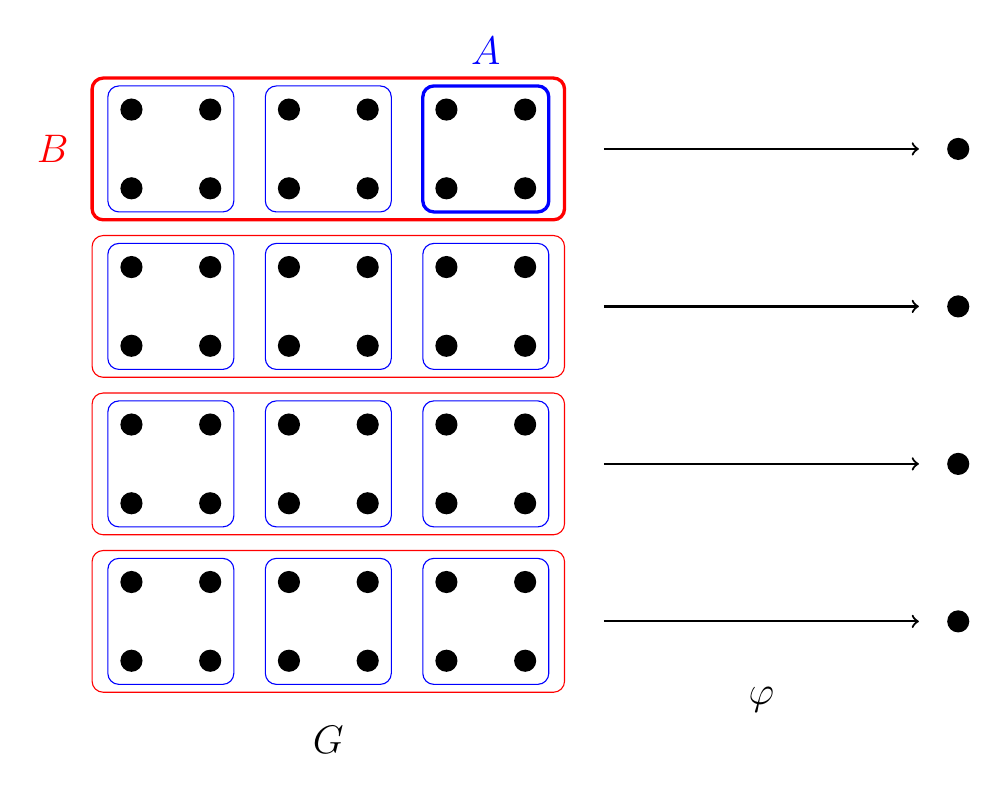
\begin{tikzpicture}
		% elements of G
		\foreach \x in {0,...,5}
		\foreach \y in {0,...,7}
		{
			\fill (\x+0.5,\y+0.5) circle (4pt);
		}
		% cosets of B
		\foreach \y in {0,...,3}
		{
			\draw[rounded corners, red] (0,2*\y+0.1) rectangle (6,2*\y+1.9);
		}
		% cosets of A
		\foreach \x in {0,...,2}
		\foreach \y in {0,...,3}
		{
			\draw[rounded corners, blue] (2*\x+0.2,2*\y+0.2) rectangle (2*\x+1.8,2*\y+1.8);
		}
		% bold subgroups A and B
		\draw[rounded corners, very thick, red] (0,6.1) rectangle (6,7.9);
		\draw[rounded corners, very thick, blue] (4.2,6.2) rectangle (5.8,7.8);
		% arrows of \varphi
		\foreach \x in {0,...,3}
		{
			\draw[->, thick] (6.5,2*\x+1) -- (10.5,2*\x+1);
		}
		\node at (8.5,0) {\Large{$\varphi$}};
		% elements of H
		\foreach \x in {0,...,3}
		{
			\fill (11,2*\x+1) circle (4pt);
		}
		% other labels
		\node at (3,-0.5) {\Large{$G$}};
		\node[blue] at (5,8.25) {\Large{$A$}};
		\node[red] at (-0.5,7) {\Large{$B$}};
	\end{tikzpicture}
\end{center}

\section{third-2}
\begin{center}
	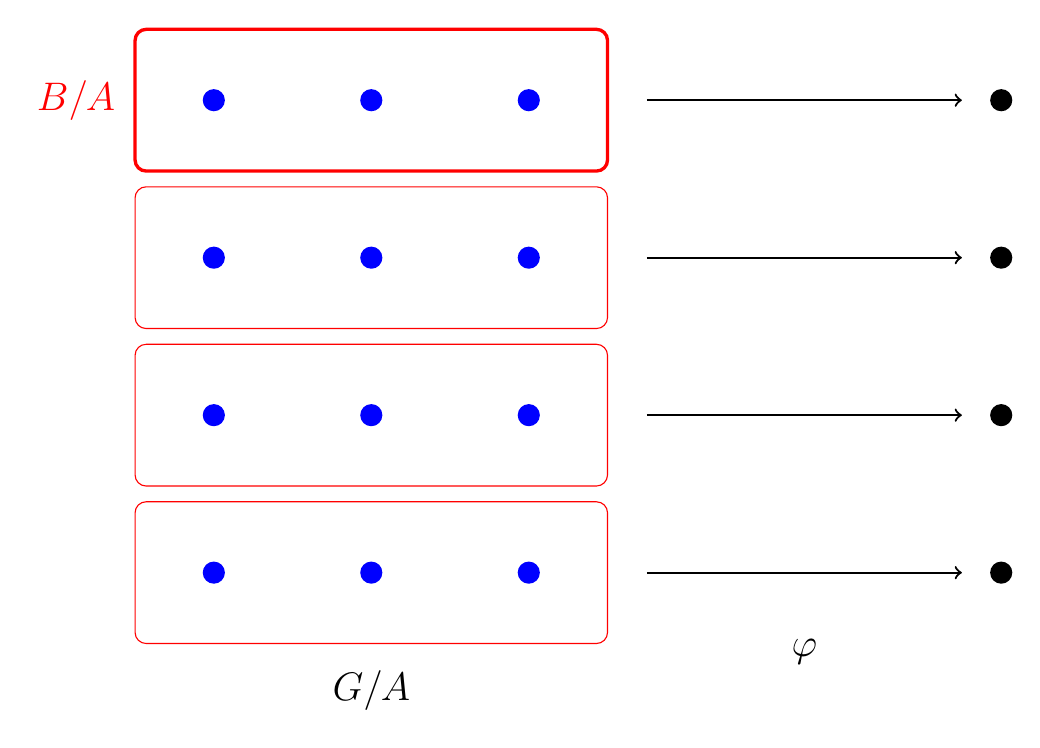
\begin{tikzpicture}
		% cosets of B
		\foreach \y in {0,...,3}
		{
			\draw[rounded corners, red] (0,2*\y+0.1) rectangle (6,2*\y+1.9);
		}
		% cosets of A
		\foreach \x in {0,...,2}
		\foreach \y in {0,...,3}
		{
			\fill[blue] (2*\x+1,2*\y+1) circle (4pt);
		}
		% bold subgroup B
		\draw[rounded corners, very thick, red] (0,6.1) rectangle (6,7.9);
		% arrows of \varphi
		\foreach \x in {0,...,3}
		{
			\draw[->, thick] (6.5,2*\x+1) -- (10.5,2*\x+1);
		}
		\node at (8.5,0) {\Large{$\varphi$}};
		% elements of H
		\foreach \x in {0,...,3}
		{
			\fill (11,2*\x+1) circle (4pt);
		}
		% other labels
		\node at (3,-0.5) {\Large{$G/A$}};
		\node[red] at (-0.75,7) {\Large{$B/A$}};
	\end{tikzpicture}
\end{center}
\end{document}
